\createTitlePage{فصل دوم}{درک صحنه}
\subsection{درک صحنه}
درک صحنه یکی از چالش‌های اساسی در زمینه بینایی ماشین است که روش‌های مختلفی برای دست‌یابی به آن ارائه شده است. با وجود تعدد پژوهش‌های موجود در این مورد، ارائه تعریف جامع و شامل برای این مفهوم کاری بسیار دشوار است. عموما این مفهوم، بسته به مورد کاربرد و هدف پژوهش، به استخراج مجموعه مشخصی از اطلاعات در مورد صحنه که برای پژوهش، کافی و مفید باشد محدود می‌شود. به همین دلیل، مجموعه اطلاعات مطلوب از تصویر که باید استخراج شود در هر پژوهش به طور خاص تعریف می‌شود.
\\
درک صحنه در زمینه تولید خودکار شرح بر تصاویر، به طور عام شامل موارد زیر می‌شود:
\begin{enumerate}
\item تشخیص اجسام موجود در صحنه و دسته‌بندی آن‌ها (مانند توپ، تلویزیون)
\item تشخیص ارتباط مکانی بین اجسام موجود در صحنه (مانند پشت، بالا)
\item دسته‌بندی محیط (مانند جنگل، دریا)
\item دسته‌بندی فعالیت به تصویر کشیده شده (مانند راه‌رفتن، خوابیدن)
\end{enumerate}

%%%%%%%%%%%%%%%%%%%%%%%%%%%%%%%%%%%%%%%%%
\subsection{روش‌های مختلف موجود}
فعالیت‌های متعددی برای تشخیص هر یک از موارد بالا انجام شده است. به طور عام می‌توان روش‌های مورد استفاده در استخراج اطلاعات مطلوب صحنه را در زمینه تولید خودکار شرح بر تصاویر به دو دسته عمده زیر تقسیم‌بندی نمود:

\begin{enumerate}
\item استفاده از مدل‌های گرافی احتمالی\enfootnote{Probabilistic Graphical Models (PGMs)} \\

در این دسته از روش‌ها، با استفاده از مدل‌های گرافی احتمالی در مورد حضور یا عدم حضور اجسام مختلف در صحنه و رابطه بین اجسام موجود استنتاج نمود. همین‌طور فرایند‌هایی مانند قطعه‌بندی تصویر\enfootnote{Image Segmentation}
در این روش‌ها با استفاده از مدل‌های گرافی احتمالی انجام می‌شوند. به عنوان نمونه، در مقاله
\cite{fidler2013sentence}
 یک مدل میدان تصادفی شرطی\enfootnote{Conditional Random Field (CRF) }
  برای تجزیه معنایی\enfootnote{Semantic Parsin
  g} تصویر ارائه شده است که با استفاده از آن می­‌توان در مورد حضور یا عدم حضور اجسام مختلف به طور توام در صحنه تصمیم­گیری کرد.
\item استفاده از شبکه‌های عصبی کانولوشنی عمیق
در این دسته از روش‌ها، با استفاده از شبکه‌های عصبی کانولوشنی عمیق، پس از قطعه‌بندی تصاویر، اقدام به تفکیک اجسام مختلف در صحنه و برچسب‌گذاری هر جسم، بسته به یادگیری انجام شده، می‌شود. به عنوان نمونه در مقاله
\cite{karpathy2015deep}
 یک شبکه عصبی کانولوشنی عمیق معرفی شده است که قادر به برچسب‌گذاری اجسام مختلف در صحنه است. برچسب‌های مورد استفاده در این پژوهش، عبارات مختلف موجود در جملات توصیف‌گر هر تصویر در مجموعه‌دادگان هستند.

\end{enumerate}

نمونه‌های متعددی از این دست پژوهش‌ها، در هر دسته، انجام شده است که در ادامه چند مورد از آن‌ها بررسی خواهد شد.

%%%%%%%%%%%%%%%%%%%%%%%%%%%%%%%%%%%%%%%%%
\subsection{روش‌های مبتنی بر مدل‌های گرافی احتمالی}

همان‌طور که قبلا ذکر شد، روش‌های مبتنی بر استفاده از مدل‌های گرافی احتمالی، از جمله پرکاربردترین روش‌ها در مرحله درک صحنه در زمینه تولید خودکار شرح بر تصاویر هستند. این روش‌ها با استفاده از نظریه گراف، آمار و احتمالات اقدام به ارائه یک توزیع احتمالی برای پارامتر مورد بررسی، با توجه به داده‌های موجود در مجموعه آموزشی می‌کنند. مدل‌های استاندارد مختلفی در پژوهش‌ها مورد استفاده قرار می‌گیرند که تعدادی از آن‌ها به عنوان نمونه در این بخش مورد بررسی قرار خواهند گرفت.
\subsubsection[استفاده از مدل میدان تصادفی مارکف]{استفاده از مدل میدان تصادفی مارکف\enfootnote{Markov Random Field (MRF)}}
مقاله
\cite{Farhadi2010every}
با استفاده از یک مدل ساده میدان تصادفی مارکف، فرایند درک صحنه را انجام می‌دهد و با استفاده از همین مدل، اقدام به تولید جملات توصیف‌گر تصویر می‌نماید. در این فصل به بررسی فرایند درک صحنه در این مقاله می‌پردازیم و بررسی فرایند تولید جمله را به فصل بعدی موکول می‌نماییم.
\\
درک صحنه در این پژوهش محدود به ارتباط بین سه مفهوم در هر تصویر شده است؛ به این معنی که به ازای هر تصویر، یک سه‌تایی «جسم، فعالیت، صحنه»\enfootnote{<Object, Activity, Scene>}
ایجاد می‌شود که بیان‌کننده اطلاعات مطلوب موجود در تصویر است. میدان\enfootnote{Field} «جسم»، دربر دارنده‌ برچسب حاصل از دسته‌بندی اجسام موجود در صحنه، میدان «فعالیت»، دربر دارنده اطلاعات مربوط به فعالیت در حال انجام و میدان «صحنه» دربردارنده اطلاعات مربوط به محیط تصویر هستند. به فضای سه‌تایی‌های ایجاد شده برای اطلاعات مطلوب در درک صحنه، فضای معنا\enfootnote{Meaning Space} می‌گویند.
\\
شکل
\ref{fig:F2010EF1}
نمایی از نگاشت اطلاعات از فضای تصاویر و جملات به فضای معنایی، نمایش می‌دهد. همان‌طور که در شکل مشخص است، به ازای هر تصویر، یک سه‌تایی معنایی ایجاد می‌شود. همین‌طور به ازای هر جمله در فضای جملات، یک سه‌تایی ایجاد می‌شود به‌طوری‌که جملات و تصاویر متناظرشان، به یک سه‌تایی یکسان، نگاشت شوند. همان‌طور که مشخص است، با داشتن نگاشت‌هایی  که خواص مذکور را داشته‌باشند، می‌توان با استفاده از سه‌تایی‌های فضای معنا، تصاویر را مدیریت کرد.

\begin{figure}[h]
\center
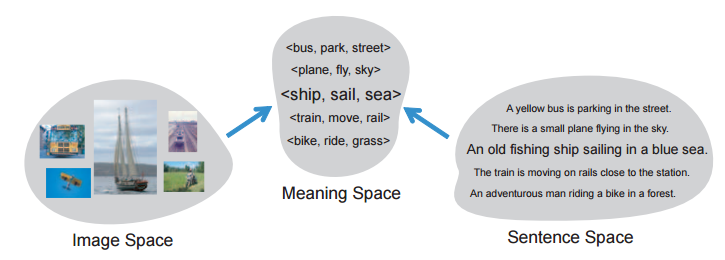
\includegraphics[scale=0.7]{./Imgs/farhadi2010every_fig1.png}
\caption{
نگاشت تصویر به فضای معنایی. فضای معنایی شامل اطلاعات مطلوب برای استخراج در فرایند درک صحنه است. به ازای هر تصویر، یک سه‌تایی ایجاد می‌شود\cite{Farhadi2010every.}
}
\label{fig:F2010EF1}
\end{figure}

مدل میدان تصادفی مارکف مورد استفاده در این پژوهش، یک مدل کوچک و ساده، شامل ۳ گره است. شکل \ref{fig:F2010EF2}
طرح‌واره‌ای از مدل میدان تصادفی مارکف مورد استفاده در این پژوهش را نمایش می‌دهد. همان‌طور که در شکل مشخص است،  به ازای هر کدام از میدان‌های تعریف شده در فضای معنایی، یک گره در این مدل وجود دارد. مقادیر مختلف در هر گره، برابر است با مقادیر مختلف موجود در میدان متناظر، در فضای معنا که با توجه به داده‌های مجموعه‌‌ ‌آموزشی مشخص می‌شوند. همین‌طور به ازای هر دو گره موجود در این مدل، یک یال بیان‌کننده ارتباط بین دو میدان در فضای معنایی وجود دارد.

برای استنتاج در این مدل، لازم است ابتدا فاکتور‌های مورد استفاده در مدل را شناخته و مقادیر آن‌ها را مشخص نماییم. در مدل پیشنهادی، دو نوع فاکتور تعریف شده است:

\begin{enumerate}
\item فاکتورهای گره\\
این فاکتورها، برای مشخص کردن میزان شباهت مقادیر مختلف گره با تصویر ورودی، تعریف شده‌‌اند. ویژگی‌‌های مورد استفاده برای مقداردهی این فاکتورها، شامل موارد زیر هستند:
\begin{enumerate}
	\item	 استفاده از آشکارکننده‌های\enfootnote{Detector}
	فلزنسوالب\enfootnote{Felzenszwaalb}، 
	به منظور محاسبه امتیاز اطمینان\enfootnote{Confidence Score} برای هر دسته از اجسام موجود در مجموعه‌داده\cite{felzenszwalb2008discriminatively}.\\
	پس از محاسبه امتیاز اطمینان همه دسته‌های موجود، دسته‌ای که بیشترین امتیاز را دارد می‌تواند به عنوان دسته‌ منتخب در میدان متناظر گره، انتخاب شود. در فرایند مقداردهی این ویژگی، قبل از انجام محاسبات، اطمینان حاصل می‌شود که از هر دسته موجود، حداقل یک تصویر در مجموعه‌داده وجود داشته باشد.
	\item استفاده از پاسخ دسته‌بندی‌کننده دیوالا\enfootnote{divvala}، ارائه شده در مقاله\cite{divvala2009empirical}
	\item استفاده از دسته‌بندی‌کننده مبتنی بر گیست\cite{Gist-based classification response}
\end{enumerate}

\begin{figure}[h]
\center
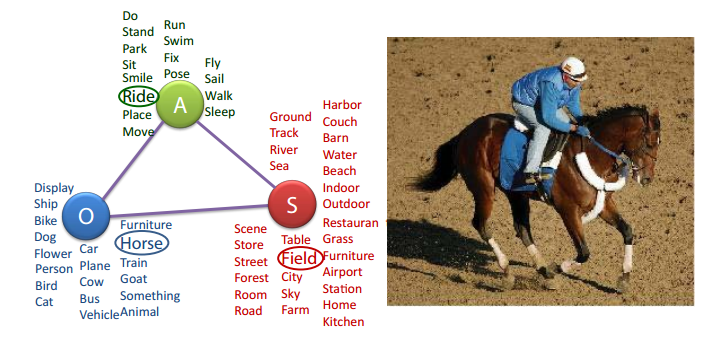
\includegraphics[scale=0.7]{./Imgs/farhadi2010every_fig2.png}
\caption{
طرح‌واره مدل میدان تصادفی مارکف ارائه شده در پژوهش \cite{Farhadi2010every} که شامل ۳ گره است. در این مدل، به ازای هر میدان از فضای معنا، یک گره وجود دارد و بین هر سه گره‌، به طور دو به دو، یک یال موجود است\cite{Farhadi2010every}.
}
\label{fig:F2010EF2}
\end{figure}

بر اساس مقادیر محاسبه شده برای ویژگی‌های بالا و با استفاده از الگوریتم ماشین بردار پشتیبان\enfootnote{Support Vector Machine (SVM)}، یک دسته‌بندی برای هر گره ارائه می‌شود که بیان‌کننده دسته‌ویژگی‌های مربوط به مقادیر مختلف گره است. با استفاده از این دسته‌بندی، با ورود هر تصویر، می‌توان برای هر مقدار در هر گره، یک امتیاز شباهت محاسبه نمود. استفاده از الگوریتم یافتن نزدیک‌ترین همسایه‌های موجود برای هر تصویر ورودی، بر اساس امتیاز شباهت محاسبه‌شده و میانگین‌گیری روی همسایه‌های استخراج شده، معیار خوبی از تخمین مقدار هر گره، به ازای هر تصویر ورودی ایجاد می‌کند. به این ترتیب، با ورود هر تصویر می‌توان برای هر کدام از گره‌های موجود در مدل، یک مقدار محتمل مشخص نمود. سه‌تایی شامل مقادیر محتمل بدست‌آمده در هر گره، سه‌تایی متناظر تصویر ورودی در فضای معنا را مشخص می‌کند.
\item فاکتورِ یال\\
این فاکتور، برای مشخص کردن میزان ارتباط مقادیر مختلف دو گره با یکدیگر در تصویر ورودی مورد استفاده قرار می‌گیرند.
\end{enumerate}

%%%%%%%%%%%%%%%%%%%%%%%%%%%%%%%%%%%%%%%%%
\subsubsection[استفاده از مدل میدان تصادفی شرطی]{استفاده از مدل میدان تصادفی شرطی\enfootnote{Conditional Random Field (CRF)}}
در این پژوهش، مساله درک صحنه در قالب یک مساله استنتاج با استفاده از مدل میدان تصادفی شرطی بیان شده است. مدل میدان تصادفی شرطی، یکی از پرکاربردترین مدل‌های گرافی احتمالی در زمینه درک صحنه است که پژوهش‌های متعددی از آن به عنوان مدل اصلی در درک صحنه استفاده کرده‌اند. به عنوان نمونه، در مقاله‌های 
\cite{Lin_2013_ICCV}
و
\cite{ladicky2010and}
از مدل میدان تصادفی شرطی به منظور توصیف صحنه استفاده شده است.\\

 پژوهش \cite{Lin_2013_ICCV} سعی در توصیف اجسام سه‌بعدی با استفاده از قطعه‌بندی تصاویر دوبعدی، هندسه سه‌بعدی و روابط بین صحنه و اجسام موجود، دارد. در این پژوهش، پس از استخراج ویژگی‌ها و اطلاعات بدست‌آمده از منابع مختلف، عمل استنتاج توسط یک مدل تصادفی شرطی انجام می‌شود که منجر به نگاشت تصویر ورودی به فضای معنایی می‌شود. همین‌طور در پژوهش \cite{ladicky2010and}، یک چارچوب کاری\enfootnote{Framework} احتمالی برای استنتاج درباره نواحی مختلف تصویر، اجسام موجود و ویژگی‌های مختلف آن‌ها مانند دسته‌بندی، موقعیت مکانی و ابعاد، مبتنی بر مدل میدان تصادفی شرطی، ارائه شده است. با توجه به وسعت و تعدد فعالیت‌های انجام شده، در این بخش، مرحله درک صحنه یک پژوهش انجام شده در زمینه تولید خودکار شرح بر تصاویر را مورد بررسی قرار می‌دهیم. لازم به ذکر است، مرحله تولید جملات توصیف‌کننده پژوهش مورد بحث، در فصل تولید جملات زبان طبیعی مورد بررسی قرار خواهد گرفت.
\\
در پژوهش\cite{fidler2013sentence}
از مدل میدان تصادفی شرطی برای توصیف صحنه و اجسام موجود در آن استفاده شده است. میدان‌های تصادفی در این مدل، شامل متغیرهای زیر هستند:
\begin{enumerate}
\item  متغیرهای تصادفی بیان‌کننده برچسب دسته متناظر قطعات مختلف هر تصویر به شیوه سلسله مراتبی دارای دو سطح
\item متغیرهای تصادفی باینری بیان‌کننده صحت دسته‌ تشخیص داده‌شده برای هر جسم
\end{enumerate}

شکل
\ref{fig:F2013SF1}
 طرح‌واره مدل سلسله‌مراتبی ارائه شده در پژوهش \cite{fidler2013sentence} را نمایش می‌دهد. همان‌طور که مشاهده می‌شود این مدل از دو سطح انتزاع، یکی برای برچسب قطعات مختلف تصویر و دیگری برای حضور یا عدم حضور هر دسته از اجسام در تصویر، تشکیل شده است.

\begin{figure}[h]
\center
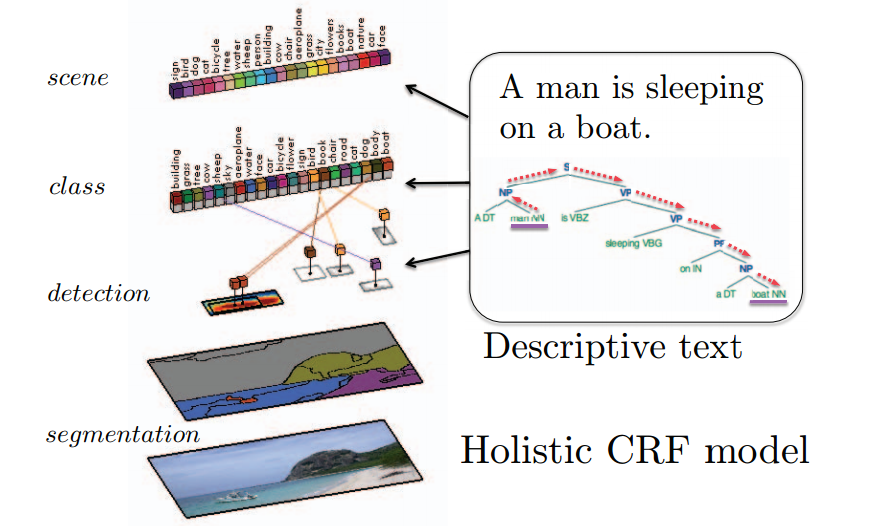
\includegraphics[scale=0.5]{./Imgs/fidler2013sentence_f1.png}
\caption{طرح‌واره مدل سلسله مراتبی مبتنی بر میدان تصادفی شرطی که بر اساس اطلاعات بصری و اطلاعات جملات توصیف‌کننده شرح محتمل تصویر را تولید می‌نماید\cite{fidler2013sentence}.}
\label{fig:F2013SF1}
\end{figure}

دو دسته متغیر تصادفی مختلف، که هر یک نماینده متغیرهای تصادفی موجود در یکی از این سطوح انتزاع هستند، تعریف شده‌اند؛ 
متغیرهای تصادفی $X_i \in {1, \cdots,C}$ بیان‌کننده دسته قطعه $i$ام از سطح پایین سلسله مراتب و متغیرهای تصادفی $Y_j \in {1, \cdots,C}$ بیان‌کننده دسته قطعه $j$ام از سطح بالای سلسله مراتب.
به علاوه، دو دسته متغیر تصادفی دیگر به نام‌های $b_l$ و $z_k$ به ترتیب برای نمایش حضور یا عدم حضور یک تشخیص کاندید\enfootnote{Candidate Detection} و حضور یا عدم حضور جسم با دسته $k$ در تصویر، تعریف شده‌اند. با توجه به متغیرهای تعریف شده، مدل کلی میدان تصادفی شرطی را می‌توان معادل رابطه\ref{eq:crffidler} تعریف کرد. در این رابطه $\Psi_\alpha^{type}(a_\alpha)$ نماینده تابع پتانسیل تعریف شده روی متغیرهای مختلف است. با این تعریف، یافتن تخمین \lr{MAP}\enfootnote{MAP Estimation}، منجر به یافتن پاسخ مورد نظر می‌شود.
در ادامه، توابع پتانسیل مختلف که در این پژوهش تعریف شده‌اند، ارائه خواهد شد. لازم به ذکر است در تمام این موارد، برای سهولت، توابع پتانسیل به شکل لگاریتمی تعریف شده‌اند.
\begin{equation}
P(X,Y,b,z) = \frac{1}{Z} \mathlarger{\mathlarger{\Pi}}_{type} \mathlarger{\mathlarger{\Pi}}_\alpha \Psi_\alpha^{type}(a_\alpha)
\label{eq:crffidler}
\end{equation}

توابع پتانسیل مختلف تعریف شده در این پژوهش عبارتند از:

\begin{enumerate}
\item پتانسیل قطعه‌بندی یگانی\enfootnote{Unary Segmentation Potential}\\
پتانسیل قطعه‌بندی یگانی در هر قطعه و هر ابرقطعه\enfootnote{Supersegment} از تصویر، با استفاده از میانگین‌گیری روی امتیاز افزایش تکستون\enfootnote{Texton Boost} که در پژوهش \cite{ladicky2010graph} ارائه شده است، انجام می‌شود.
\item انطباق بین متغیرهای دو سطح انتزاع با یک‌دیگر\\
یک مقدار جریمه به ازای دسته‌های مخالف بین دو سطح در نظر گرفته‌ می‌شود تا در حد امکان، دسته‌های منتخب از بین سطوح مختلف، با یک‌دیگر انطباق داشته باشند. پتانسیل تعریف شده در این بخش معادل رابطه\ref{eq:phiijf} 
تعریف می‌شود.
	\begin{equation}
		\phi_{ij}(X_i, Y_j)=
			\left\{
				\begin{array}{ll}
					- \gamma		&	X_i \neq Y_j \\
					0			&	X_i	=	Y_j
				\end{array}							
			\right.
		\label{eq:phiijf}
	\end{equation}
در رابطه\ref{eq:phiijf}، پارامتر $\gamma$ در فرآیند یادگیری که منجر به بهینه‌سازی پارامترهای مختلف مدل می‌شود، به‌دست می‌آید.
\item پتانسیل انطباق تصویر و دسته جسم\\
برای اندازه‌گیری میزان انطباق هر کدام از دسته‌های موجود برای اجسام با تصویر ورودی، از معیار انطباق ارائه شده در پژوهش\cite{felzenszwalb2010object}
 توسط فلزنسوالب که به روش دی پی ام\enfootnote{DPM} مشهور است، استفاده شده است. برای کاهش تعداد پارامترها و افزایش کارایی مدل استفاده شده، برای هر تصویر حداکثر ۳ دسته جسم، به عنوان دسته‌های منتخب کاندید، در نظر گرفته می‌شوند.
\end{enumerate}


%%%%%%%%%%%%%%%%%%%%%%%%%%%%%%%%%%%%%%%%%
\subsubsection{استفاده از سایر مدل‌های گرافی احتمالی}
در بین پژوهش‌های موجود در زمینه درک صحنه با استفاده از روش‌های احتمالاتی، علاوه بر مدل‌های استاندارد، از مدل‌های مولد دیگر در پژوهش‌های متعددی استفاده شده است. در ادامه این بخش، به بررسی چند‌ نمونه از این مدل‌ها خواهیم پرداخت.

\begin{enumerate}
\item دسته‌بندی تصاویر بر اساس صحنه و اجسام موجود به طور توام\cite{li2007and}

مدل استفاده شده در این پژوهش، از تصاویر در سطح صحنه و سطح اجسام استفاده کرده و با یکپارچه‌سازی و تجمیع اطلاعات موجود در این دو سطح، اقدام به دسته‌بندی تصویر می‌نماید. شکل\ref{fig:l2007af1} 
مدل استفاده شده در این پژوهش را به منظور یکپارچه‌سازی و تجمیع اطلاعات حاصل از تحلیل صحنه و تشخیص اجسام موجود در آن، ارائه می‌دهد.


\begin{figure}[H]
\center
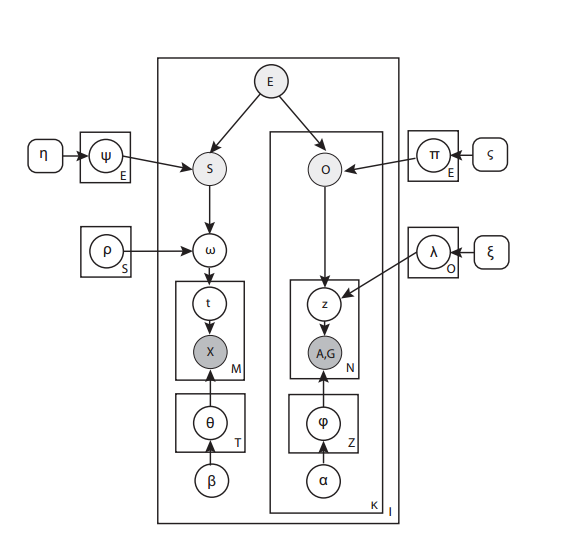
\includegraphics[scale=0.5]{./Imgs/li2007and_model.png}
\caption{مدل استفاده شده به منظور تجمیع اطلاعات صحنه و اجسام موجود در آن به منظور دسته‌بندی تصاویر\cite{li2007and}}
\label{fig:l2007af1}
\end{figure}

یکی از اهدافی که در این پژوهش دنبال می‌شود، برچسب‌گذاری معنایی\enfootnote{Semantic Labelling} تمام پیکسل‌های موجود در تصویر است. به همین منظور، تمام تصاویر مورد استفاده، به نواحی $10 * 10$ تقسیم شده و مورد استفاده قرار می‌گیرند. برای بررسی بهتر مدل، ابتدا متغیرهای تصادفی مورد استفاده را تعریف کرده و سپس به بررسی روند یادگیری و استنتاج مدل می‌پردازیم.
\\
متغیر تصادفی $X$ که حاوی اطلاعاتی مبتنی بر حضور یا عدم حضور دسته‌های مختلف صحنه است، در بخش تشخیص صحنه به‌کار می‌رود. اطلاعات این متغیر با استفاده از توصیف‌کننده سیفت\enfootnote{SIFT Descriptor} و به ازای هر ناحیه از تصویر، به‌دست می‌آید. برای بخش تشخیص اجسام موجود در صحنه، از دو منبع اطلاعاتی مختلف استفاده می‌شود. اطلاعات مربوط به حضور یا عدم حضور دسته‌های مختلف اجسام در متغیر تصادفی $A$ و اطلاعات مربوط به شکل کلی آن‌ها در متغیر تصادفی $G$ نمایش داده‌ می‌شود.
\\
هر گره از مدل ارائه شده، نماینده یک متغیر تصادفی است. گره‌هایی که با رنگ تیره مشخص شده‌اند، نماینده متغیرهایی هستند که در فرایند آموزش دیده می‌شوند و بقیه متغیرها، متغیرهای مخفی\enfootnote{Latent} هستند. گره‌های خاکستری روشن‌تر، متغیرهایی هستند که فقط در فرایند آموزش دیده‌ می‌شوند در حالی‌که متغیرهای تیره‌تر در هر دو فرایند آموزش و آزمون مشاهده می‌شوند.
\\
متغیر تصادفی $E$، نماینده یک دسته‌ از رخداد
\enfootnote{Event}
های ممکن است. توزیع احتمال اولیه این متغیر  تصادفی، یک توزیع یکنواخت فرض شده است که به هر تصویر ورودی، بر اساس همین توزیع، یک مقدار خاص از این متغیر تصادفی اختصاص داده می‌شود. با دانستن دسته رخداد موجود در تصویر، یک تصویر صحنه\enfootnote{Scene Image} متناظر با تصویر ورودی تولید می‌شود. با فرض وجود $S$ دسته صحنه مختلف در مجموعه‌داده، به هر تصویر، تنها یک دسته صحنه اختصاص داده می‌شود. روند اختصاص دسته صحنه به تصویر مطابق زیر است:
\begin{itemize}
\item[*]
ابتدا یک دسته اولیه مطابق با توزیع احتمال شرطی 
$P(S|E, \psi)$
به تصویر اختصاص داده می‌شود. $\psi$ یک پارامتر چندجمله‌ای
\enfootnote{Multinomial}
 حاکم بر توزیع احتمالاتی $S$ به شرط داشتن $E$ است. به علاوه، $\psi$ یک ماتریس به ابعاد $E * S$ و پارامتر $\eta$ یک بردار $S$ بعدی در نقش مقدار اولیه دیریکله
\enfootnote{Dirichlet prior}
 برای پارمتر $\psi$ است.
\item[*]
در قدم بعدی با داشتن مقدار $S$، پارامترهای $\omega$ را بر اساس احتمال 
$P(\omega|S, \rho)$
تولید می‌کنیم. از آن‌جا که $\omega$ پارامتر چندجمله‌ای گره‌های مخفی $t$ هستند، باید مجموع همه آن‌ها برابر با یک باشد. به علاوه، $\rho$ یک ماتریس به ابعاد $S * T$ و مقدار اولیه دیریکله برای پارامتر $\omega$ است که در آن $T$ تعداد کل $t$ها است.
\item[*] 
برای تولید هر یک از $M$ ناحیه تصویر (مقادیر متغیر تصادفی $X$) به شکل زیر عملی می‌کنیم:
\begin{itemize}
\item[-]
یک مقدار $t$ از توزیع احتمال $Mult(\omega)$ تولید می‌شود که مشخص‌کننده موضوعی\enfootnote{Topic} است که این ناحیه از تصویر مطابق با آن تولید شده است.
\item[-]
متغیر تصادفی $X$ از توزیع احتمالی $P(X$

\end{itemize}
\end{itemize}



\item درک صحنه بر اساس نواحی مختلف تصویر، اجسام موجود و روابط سه‌بعدی بین ‌آن‌ها\cite{gould2009decomposing}
\end{enumerate}

%%%%%%%%%%%%%%%%%%%%%%%%%%%%%%%%%%%%%%%%%
\subsection{روش‌های مبتنی بر شبکه‌های عصبی کانولوشنی عمیق}
